%%
%% The original source files were:
%%
%% samples.dtx  (with options: `all,proceedings,bibtex,manuscript')
%% 
%% IMPORTANT NOTICE:
%% 
%% For the copyright see the source file.
%% 
%% Any modified versions of this file must be renamed
%% with new filenames distinct from sample-manuscript.tex.
%% 
%% For distribution of the original source see the terms
%% for copying and modification in the file samples.dtx.
%% 
%% This generated file may be distributed as long as the
%% original source files, as listed above, are part of the
%% same distribution. (The sources need not necessarily be
%% in the same archive or directory.)
%%
%%
%% Commands for TeXCount
%TC:macro \cite [option:text,text]
%TC:macro \citep [option:text,text]
%TC:macro \citet [option:text,text]
%TC:envir table 0 1
%TC:envir table* 0 1
%TC:envir tabular [ignore] word
%TC:envir displaymath 0 word
%TC:envir math 0 word
%TC:envir comment 0 0
%%
%% The first command in your LaTeX source must be the \documentclass
%% command.
%%
%% For submission and review of your manuscript please change the
%% command to \documentclass[manuscript, screen, review]{acmart}.
%%
%% When submitting camera ready or to TAPS, please change the command
%% to \documentclass[sigconf]{acmart} or whichever template is required
%% for your publication.
%%
%%
\documentclass[manuscript,screen,review]{acmart}
% Chinese body (compile with XeLaTeX / LuaLaTeX)
\usepackage[UTF8,scheme=plain]{ctex}


\usepackage{algorithm}
% Use algorithmicx + algpseudocode: provides \Require, \Ensure, \State, and \Comment
\usepackage{algorithmicx}
\usepackage{algpseudocode}
% Provide compatibility shims for uppercase macros used in the document
% Some authors use \REQUIRE/\ENSURE/\UPON/\ENDUPON (uppercase) — map them to algpseudocode
\providecommand{\REQUIRE}[1]{\Require{#1}}
\providecommand{\ENSURE}[1]{\Ensure{#1}}
% \UPON{<cond>} will render as a bold 'Upon <cond>' state line inside algorithmic blocks
\providecommand{\UPON}[1]{\State\textbf{Upon}~#1}
\providecommand{\ENDUPON}{}
\providecommand{\Upon}[1]{\State\textbf{Upon}~#1}
\providecommand{\EndUpon}{}
% Provide uppercase aliases commonly used in algorithm blocks
\providecommand{\STATE}{\State}
\providecommand{\COMMENT}[1]{\Comment{#1}}
% Map common uppercase algorithmic keywords to algorithmicx/algpseudocode commands
\providecommand{\IF}{\If}
\providecommand{\ELSE}{\Else}
\providecommand{\ELSIF}{\ElsIf}
\providecommand{\ENDIF}{\EndIf}
\providecommand{\FOR}{\For}
\providecommand{\ENDFOR}{\EndFor}
\providecommand{\WHILE}{\While}
\providecommand{\ENDWHILE}{\EndWhile}
\providecommand{\RETURN}{\State\textbf{return}~}
\usepackage{tikz}
% Load common tikz libraries used in figures (positioning provides the "of" syntax)
\usetikzlibrary{positioning,arrows.meta,calc,shapes,shadows}
% color support for \textcolor used inside algorithms
\usepackage{xcolor}
% Math packages required for \text and bold symbols inside math
\usepackage{amsmath}
\usepackage{bm}
\usepackage{adjustbox}
% Define common math operators used in the document
\DeclareMathOperator*{\argmin}{arg\,min}
\DeclareMathOperator*{\argmax}{arg\,max}
\usepackage{multirow}
\usepackage{booktabs}
% Enable list customization (leftmargin, itemsep, etc.) used in the document
\usepackage{enumitem}
\newlength{\tblwidth}
\setlength{\tblwidth}{\linewidth}
% Ensure header height is sufficient for fancyhdr
\setlength{\headheight}{20.48303pt}
% theorem environments used in the document
\usepackage{amsthm}
\newtheorem{theorem}{Theorem}
\newtheorem{definition}{Definition}
\newtheorem{assumption}{Assumption}
\newtheorem{proposition}{Proposition}
\newtheorem{problem}{Problem}
\newtheorem{lemma}{Lemma}
\newtheorem{corollary}{Corollary}
\newtheorem{remark}{Remark}

\newenvironment{tablenotes}{%
    \par\footnotesize
    \begin{list}{}{% 
        \setlength{\leftmargin}{1.5em}%
        \setlength{\labelsep}{0.5em}%
        \setlength{\itemsep}{0pt}%
        \setlength{\parsep}{0pt}%
    }%
}{%
    \end{list}%
}

%%
%% \BibTeX command to typeset BibTeX logo in the docs
\AtBeginDocument{%
  \providecommand\BibTeX{{%
    Bib\TeX}}}

%% Rights management information.  This information is sent to you
%% when you complete the rights form.  These commands have SAMPLE
%% values in them; it is your responsibility as an author to replace
%% the commands and values with those provided to you when you
%% complete the rights form.
\setcopyright{acmlicensed}
\copyrightyear{2025}
\acmYear{2025}
\acmDOI{XXXXXXX.XXXXXXX}

%% These commands are for a PROCEEDINGS abstract or paper.
%%  \acmConference[Conference acronym 'XX]{Make sure to enter the correct
%% 	conference title from your rights confirmation email}{June 03--05,
%% 	2018}{Woodstock, NY}

%%
%%  Uncomment \acmBooktitle if the title of the proceedings is different
%%  from ``Proceedings of ...''!
%%
%%\acmBooktitle{Woodstock '18: ACM Symposium on Neural Gaze Detection,
%%  June 03--05, 2018, Woodstock, NY}
%%\acmISBN{978-1-4503-XXXX-X/2018/06}


%%
%% Submission ID.
%% Use this when submitting an article to a sponsored event. You'll
%% receive a unique submission ID from the organizers
%% of the event, and this ID should be used as the parameter to this command.
%%\acmSubmissionID{123-A56-BU3}

%%
%% For managing citations, it is recommended to use bibliography
%% files in BibTeX format.
%%
%% You can then either use BibTeX with the ACM-Reference-Format style,
%% or BibLaTeX with the acmnumeric or acmauthoryear sytles, that include
%% support for advanced citation of software artefact from the
%% biblatex-software package, also separately available on CTAN.
%%
%% Look at the sample-*-biblatex.tex files for templates showcasing
%% the biblatex styles.
%%

%%
%% The majority of ACM publications use numbered citations and
%% references.  The command \citestyle{authoryear} switches to the
%% "author year" style.
%%
%% If you are preparing content for an event
%% sponsored by ACM SIGGRAPH, you must use the "author year" style of
%% citations and references.
%% Uncommenting
%% the next command will enable that style.
%%\citestyle{acmauthoryear}


%%
%% end of the preamble, start of the body of the document source.
\begin{document}

%%
%% The "title" command has an optional parameter,
%% allowing the author to define a "short title" to be used in page headers.
\title{Kinematic Spatiotemporal Constraint-Based Detection and Adaptive Isolation of Byzantine False Messages in Industrial Multi-Agent Systems}

%%
%% The "author" command and its associated commands are used to define
%% the authors and their affiliations.
%% Of note is the shared affiliation of the first two authors, and the
%% "authornote" and "authornotemark" commands
%% used to denote shared contribution to the research.
\author{Qi Yu}
%%\authornote{.}
%%\authornotemark[1]
\email{230240012@seu.edu.cn}
%%\orcid{1234-5678-9012}
\affiliation{%
	\institution{School of Cyber Science and Engineering, Southeast University}
	\city{Nanjing}
	\state{Jiangsu}
	\country{PR China}
}


\author{Wei Li}
%%\orcid{1234-5678-9012}
\email{xchlw@seu.edu.cn}
\authornote{corresponding author}
%%\authornotemark[1]
\affiliation{%
	\institution{School of Computer Science and Engineering, Southeast University}
	\city{Nanjing}
	\state{Jiangsu}
	\country{PR China}
}


%%
%% By default, the full list of authors will be used in the page
%% headers. Often, this list is too long, and will overlap
%% other information printed in the page headers. This command allows
%% the author to define a more concise list
%% of authors' names for this purpose.

%%\renewcommand{\shortauthors}{Yu et al.}

\title{基于耦合互证与可问责沉默的被劫持设备任务状态伪造检测}
\subtitle{Detecting Task-State Falsification by Compromised Devices via Coupled Corroboration and Accountable Silence}

\renewcommand{\shortauthors}{Yu and Li}

\begin{CCSXML}
<ccs2012>
 <concept>
  <concept_id>10002978.10003006.10003013</concept_id>
  <concept_desc>Security and privacy~Intrusion detection systems</concept_desc>
  <concept_significance>500</concept_significance>
 </concept>
 <concept>
  <concept_id>10010583.10010662.10010674</concept_id>
  <concept_desc>Hardware~Safety critical systems</concept_desc>
  <concept_significance>300</concept_significance>
 </concept>
 <concept>
  <concept_id>10003033.10003083.10003095</concept_id>
  <concept_desc>Networks~Cyber-physical networks</concept_desc>
  <concept_significance>300</concept_significance>
 </concept>
</ccs2012>
\end{CCSXML}

\ccsdesc[500]{Security and privacy~Intrusion detection systems}
\ccsdesc[300]{Hardware~Safety critical systems}
\ccsdesc[300]{Networks~Cyber-physical networks}

\begin{abstract}
被劫持的现场设备可如实上报物理量、只伪造离散任务状态；此类谎言不产生物理残差，单观测者族（看门狗以外的残差、过程一致性与虚假数据注入检测）在构造上无法检出。
事件触发通信下的沉默攻击面已有文献指出，见证式位置证明多按地理邻居选人，工业心跳多只管通信活性——仍缺少用\textbf{任务耦合对手方}否证完成类谎言、以及\textbf{不依赖共识分歧}的沉默归责。
本文提出两条互补通道：由任务图导出 $O(1)$ 见证集上的耦合互证，以及哈希链锚定的可问责沉默；二者合用堵住攻击者决策树，心跳间隔 $T_{\mathrm{hb}}$ 由安全预算反解而非自选。
串谋代价由互证超图前向闭包给出结构下界；检测时延的无条件上界 $r\,T_{\mathrm{hb}}$ 接入危害模型导出的时间预算（定理只接沉默通道；运动危害仅作预算量级校准）。
在 Fischertechnik Trier 工业物联网事件日志上：同协议仅更换见证选取时，空间邻居原则约恢复 52\% 检出；谎报且维持心跳（P3）仅互证有效；最严心跳带宽约 7.7\,KB/s，约为 5\,Hz 全网 PBFT 的 $1/131$。
\end{abstract}

\keywords{任务状态伪造, 耦合互证, 可问责沉默, 工业调度, 被劫持设备, 带宽--安全权衡}

\maketitle

%=============================================================================
\section{引言}
\label{sec:introduction}

工业生产调度系统由中央调度器与一组异构现场设备构成：设备执行下行命令并上报上行状态，派工决策依赖调度器维护的\textbf{任务状态视图}。
攻击面因而落在污染该视图以骗取派工，而非攻破设备连续控制回路。
被劫持设备可以如实上报位置与运动学量，只将``完成/可用''等离散结果位翻真——此类\textbf{任务状态伪造}不产生物理残差，残差类虚假数据注入（FDI）检测、数字孪生 KPI 异常检测与单观测者计划一致性检验在构造上对其失效。

调度层同时具备若干可被检测器利用、而攻击者难以同时伪造的结构。
其一，离散任务状态可在无物理残差下伪造，单观测者可见字段甚至可与良性样本逐字段一致。
其二，任务交接是\textbf{双方物理事件}：是否交付发生，证据在诚实对手方的到料/取件等本地传感中，攻击者控制不了。
其三，合格见证者由\textbf{任务图}而非无线拓扑决定，规模为 $O(1)$ 且任务下发时已知。
其四，事件触发语义下``无完成消息''本可按预测推进，沉默因此免费——除非沉默本身被承诺为可证伪声明。
另有：互证 pending 由命令打开而非由完成声明打开；谎言要存活到物料被消耗，须沿任务链买通前向可达闭包。

\paragraph{引导例（攻击者决策树）。}
考虑 AGV--机械臂车间：调度器命令 AGV-7 将工件送至机械臂 R3 交接。
AGV-7 已被劫持，目标是骗取``已完成、我空闲''以持续套取派单。
攻击者只有四条路：（P1）谎报完成且不维持心跳；（P2）完全沉默；（P3）谎报完成但按时披露心跳原像；（P4）与对手方一跳串谋。
两条通道各有对方覆盖不到的缺口：\textbf{仅沉默}抓不住按时披露原像的谎报（P3）；\textbf{仅互证}虽因命令开窗仍能发现沉默，但时延受派发排队支配（数十～数百秒），无法给出无条件安全时延界。
\textbf{二者合用}后决策树无获胜支：说谎被对手方否证，沉默被缺失原像在约秒级判定，假称合法则自证其罪。
本文用该叙事讲清威胁；实验在 Fischertechnik Trier 日志上实例化同一形式化对象（无 AGV、无通信层处，心跳/危害预算参数另行标注来源）。
图~\ref{fig:attack-tree} 概括四路决策与对应检出通道。

\begin{figure}[t]
  \centering
  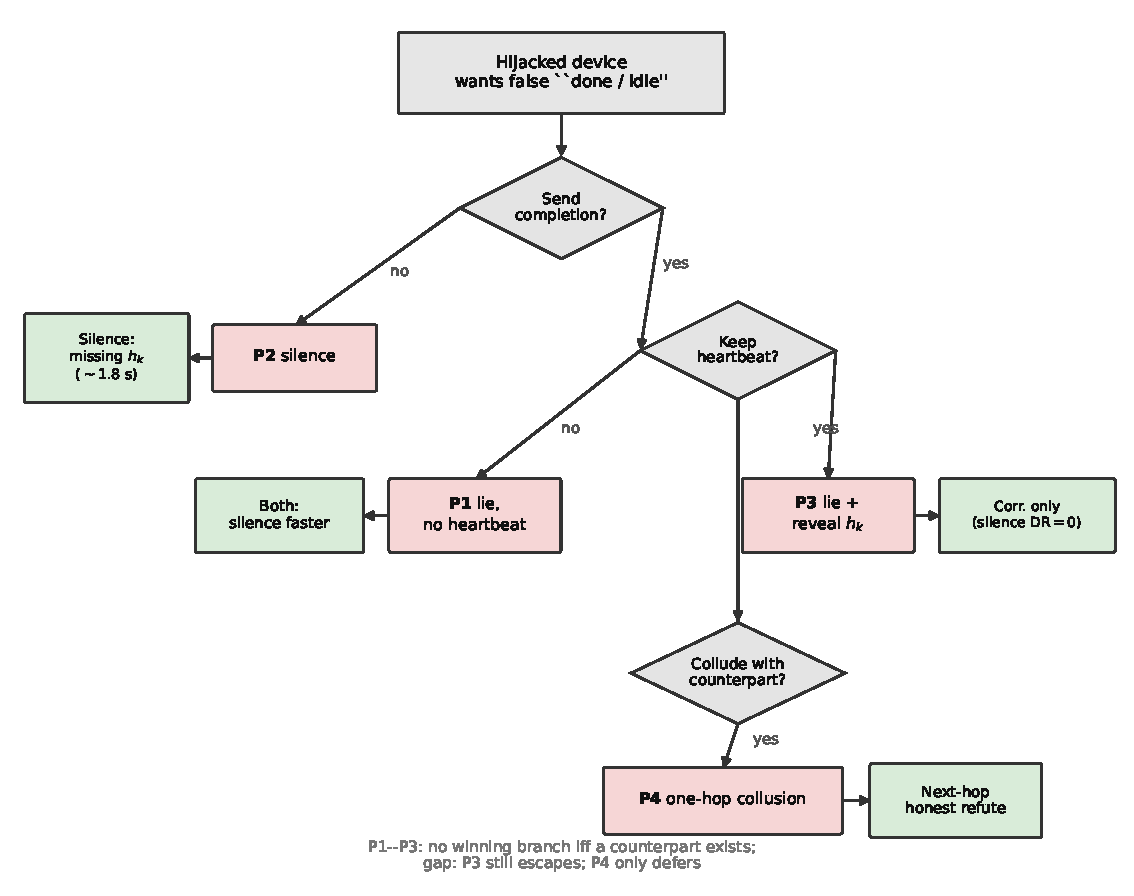
\includegraphics[width=\columnwidth]{fig/fig_attack_tree.pdf}
  \Description{Attacker decision tree with branches P1--P4 and detecting mechanisms.}
  \caption{攻击者决策树（P1--P4）。合用耦合互证与可问责沉默后无获胜支；P3 仅互证可抓。}
  \label{fig:attack-tree}
\end{figure}

\paragraph{公开缺口。}
单观测者残差/FDI 一支假定伪造会扰动连续物理量~\cite{ditof2024,dtmpc2025}；PeerReview 承认无法确定性归责``该发不发''~\cite{peerreview2007}；Polygraph/ABC 的归责绑定在共识分歧之后~\cite{polygraph2021,abc2023}；TESLA 明确不提供不可否认性~\cite{tesla2001,rfc4082}；IEC 61850 GOOSE 心跳只管通信活性；COLAW/Vouch+ 等位置证明按地理邻居选人~\cite{colaw2020,vouch2019}；DIAT 等依赖 TEE 与软件完整性~\cite{diat2019}。
仍缺的是：以任务耦合对手方否证离散完成声明，以及不依赖分歧的沉默归责。

\paragraph{贡献。}
问题设定（无残差的任务状态伪造）用于框定 Introduction，不单独计为技术贡献。本文贡献三条：
\begin{enumerate}[leftmargin=*,itemsep=2pt]
  \item \textbf{耦合互证的见证选取原则与串谋界。} 见证集由任务图诱导的互证超图导出；同协议下仅换选取规则时，空间邻居原则约恢复 52\% 检出且见证集更大，说明增量在选取原则而非``有见证者''。
  \item \textbf{可问责沉默。} 一次签名锚定的哈希链 + 有界心跳，把沉默升级为可证伪、可归因声明，给出不依赖分歧的归责路径。
  \item \textbf{带宽--安全裕度权衡。} 危害模型 $\to$ 时间预算 $\to$ 可行 $(r,T_{\mathrm{hb}})$ $\to$ 带宽；定理只接沉默通道的无条件时延上界 $r\,T_{\mathrm{hb}}$。运动碰撞危害仅用于校准预算量级，主安全论断仍是调度损害下的可检测性。
\end{enumerate}
非对称密码预算（高频 MAC/哈希链，稀有事件才用签名）作为工程附带，不作主创新头条。

第~\ref{sec:related}~节划界相关工作；第~\ref{sec:model}~节给出系统与威胁模型及覆盖矩阵；第~\ref{sec:method}~节描述方法；第~\ref{sec:theory}~节给出串谋界与带宽定理；第~\ref{sec:eval}~节报告实验；第~\ref{sec:conclusion}~节总结局限与结论。

%=============================================================================
\section{相关工作}
\label{sec:related}

\subsection{事件触发与拜占庭共识}

PISTIS 等自称事件触发的实时拜占庭协议，其``事件''是消息到达与连通性变化~\cite{pistis2021}；控制论一支则以连续状态偏差超阈为触发条件~\cite{tac2025el,hdetm2024}。
工业侧轻量 PBFT 工作多压缩单轮消息数 $M$ 与阶段数~\cite{ccgridw2023pbft,sensors2024aloha}，共识频率 $R$ 仍由外部周期决定。
本文事件位于工艺/任务语义层，优化轴明确放在 $R$；``事件触发 + BFT''大方向不新，不作为创新点。
PISTIS 不消费任务事件，不宜作本数据上的数值基线；等协议对照改由见证选取族承担。

\subsection{非触发攻击面}

文献已提出并分析利用触发机制本身的 non-triggering misbehavior~\cite{nontrigger2022}：受损智能体已偏离期望却不产生事件；相关工作亦在事件触发框架内做抗欺骗控制器综合~\cite{asjc2023contain,ijrnc2023deception}。
既有工作止于性能分析与鲁棒控制补偿，不给出``这段沉默是否合法''的可验证判定。
\textbf{攻击的学术提出权属该文献}；本文贡献是离散任务调度语境下的运行时检出与归责。

\subsection{可问责性、哈希链与工业心跳}

PeerReview 提供通用可问责层，但明确无法确定性揭发``该发不发''~\cite{peerreview2007}。
Polygraph/ABC 在分歧已发生时输出不可反驳证据~\cite{polygraph2021,abc2023}。
TESLA 用延迟密钥披露做源认证，但声明不提供不可否认性~\cite{tesla2001,rfc4082}；后续 Inf-TESLA 等仍沿用同一原语边界~\cite{inftesla2022}。
IEC~61850 GOOSE 心跳语义是通信活性（MaxTime / TAL），无密码绑定，丢失只触发 fail-safe~\cite{goose615}。
US-AID 等``不在场证明''证明的是设备物理在场，而非任务状态落在可行域~\cite{usaid}。
本文增量：在松散时间同步与有界心跳假设下，用预承诺哈希链把沉默变成确定性可归因行为，且不依赖分歧已发生。

\subsection{协作认证与见证式互证}

DIAT 等依赖 TEE/软件完整性~\cite{diat2019}；COLAW/Vouch+ 由地理邻居见证位置~\cite{colaw2020,vouch2019}；车联网集体感知亦强调多见证者冗余~\cite{etsi460}；DiToF 用数字孪生偏差相关性分类 FDI~\cite{ditof2024}。
本文见证者是任务耦合的物理对手方，见证内容是离散状态迁移是否发生；见证集由任务图预先确定，并导出串谋结构下界。

\subsection{工业调度层的逻辑状态伪造}

AGV 数字孪生 KPI、LSTM 孪生 MPC 与电网 FDI 检测等~\cite{dtmpc2025,agvkpi2022,fdi2024frontiers}共同前提是单观测者对连续物理量做残差检测；亦有专利将事件触发与多 AGV 抗 FDI 路径跟踪结合做控制补偿而非归责~\cite{cn120578205b}。
如实上报位置、只伪造任务状态的攻击不产生残差，对该族结构性免疫——这正是标题强调``任务状态''的原因。

\begin{table}[t]
  \centering
  \caption{相关工作定位（摘要）}
  \label{tab:rw}
  \begin{tabular}{@{}llp{0.38\columnwidth}@{}}
    \toprule
    方法类 & 核心前提 & 相对本文 \\
    \midrule
    残差/FDI/孪生 & 连续物理量异常 & 无残差任务伪造失效 \\
    GOOSE 式心跳 & 通信活性 & 无状态声明、无归责 \\
    Polygraph/ABC & 共识已分歧 & 沉默无分歧时不可用 \\
    地理邻居见证 & 无线拓扑选人 & 非任务耦合、$|W|$ 不可预知 \\
    \textbf{本文} & 任务图见证 + 承诺式沉默 & --- \\
    \bottomrule
  \end{tabular}
\end{table}

%=============================================================================
\section{系统模型与威胁模型}
\label{sec:model}

\subsection{系统构成与形式化对象}
\label{sec:sys}

中央调度器 $S$ 与现场设备集 $\mathcal{D}=\{d_1,\dots,d_n\}$ 经工业网络互联。
设备不自治协商：执行下行命令 $u$，上报上行声明 $r$。
$S$ 持有命令账本 $c$（已下发、未撤销的命令）；账本是调度器既有产物，\textbf{不是本文贡献}。
活动/任务实例记为 $a$；工艺模型导出任务图 $G=(V,E)$，进而导出互证超图 $H$（跨设备类、同位置的交付--取件对），见证集 $W(a)$ 由 $H$ 确定。
互证窗口 $\Delta$ 须容纳派发排队；心跳间隔 $T_{\mathrm{hb}}$ 与连续缺失判决数 $r$ 由安全预算反解。

引导例用 AGV--臂交接讲清语义；实验用 Trier 的工位交接实例化同一对象（如 VGR 交付至某位置、下游取走对应 $H$ 上的边）。

\begin{figure}[t]
  \centering
  
\includegraphics[width=\columnwidth]{fig/fig_system.pdf}
  \Description{Scheduler issues commands that open corroboration pending; devices send completion reports and heartbeat preimages; counterparts confirm or refute.}
  \caption{系统构成与消息回环：下行命令打开互证 pending；完成类声明走耦合互证，心跳原像走可问责沉默。}
  \label{fig:system}
\end{figure}

\subsection{消息回环}
\label{sec:msg}

下行 $S\!\to\!d$：命令 $u$ 入账即打开互证 pending——即便设备事后沉默，命令时刻仍存在。
上行 $d\!\to\!S$ 两类载荷分开处理：
\begin{enumerate}[leftmargin=*,itemsep=1pt]
  \item \textbf{任务完成类}（结果位、起终点、时长）$\to$ 耦合互证消费；
  \item \textbf{心跳原像类}（槽 $k$ 的哈希链元素）$\to$ 可问责沉默消费。
\end{enumerate}
事件触发下``无完成消息 $\neq$ 无命令''；看门狗能管``该报的没报''，管不住``报了但是假的''。

\subsection{威胁模型}
\label{sec:threat}

\textbf{攻击者}是被劫持的现场设备 $d\in\mathcal{D}$：$S$ 本身不被攻破。
攻击者\textbf{能够}：任意伪造或扣留上行声明；如实使用物理定位（无残差来源）；掌握过程模型与\textbf{发往本机的命令}（账本对接收方可见，攻击者比``猜最可能下一步''设定更强）；多设备串谋；造成丢包/突发丢包（影响误报口径，不改变判决语义）。
攻击者\textbf{不能}：攻破 $S$ 或改账本；凭空改变物理世界使诚实对手方``看见''未发生的交接；伪造他机哈希链原像或承诺根；在无松散时间同步假设下仍要求确定性沉默归责。

\textbf{目标}是使 $S$ 的任务状态视图与物理现实脱节（骗完成/空闲、下游饥饿等）。主危害叙事是调度损害；运动碰撞仅作危害预算量纲示意。

\textbf{根本非对称性：}攻击者控制上行声明的内容与是否发送，但不控制物理交接是否真实发生，也不控制他机原像与 $S$ 侧归档。

\begin{assumption}[显式假设]
松散时间同步（误差计入 skew）；交接相关设备具备到料/取件类本地传感（否则落入覆盖缺口）；不假设 TEE；本机命令默认可见（不做更弱知识等级）。
\end{assumption}

\subsection{攻击类型与检测通道覆盖矩阵}
\label{sec:coverage}

表~\ref{tab:coverage} 同时是威胁分类、方法必要性与消融设计依据。
数字来自 Trier 注入实验（注入率 0.2，种子 42；互证容差 260\,s）。
表中沉默时延采用检测回放口径 $r{=}9,\,T_{\mathrm{hb}}{=}0.2$\,s（中位约 1.8\,s）；第~\ref{sec:bw}~节预算求解则另解可行 $(r,T_{\mathrm{hb}})$，两套口径勿混读。
格内为检出率 / 时延中位（秒）。

\begin{table*}[t]
  \centering
  \caption{攻击类型与检测通道覆盖矩阵（DR / 时延中位）}
  \label{tab:coverage}
  \begin{tabular}{@{}lllll@{}}
    \toprule
    攻击 & 看门狗 S1 & 仅耦合互证 & 仅可问责沉默 & \textbf{合用} \\
    \midrule
    P1 谎报完成、不维持心跳 & 0.000 & 1.000 / 54.6 & 1.000 / 1.8 & \textbf{1.000 / 1.8} \\
    P2 完全沉默 & 1.000 / 334 & 0.746 / 325 & 1.000 / 1.8 & \textbf{1.000 / 1.8} \\
    P3 谎报完成且按时披露原像 & 0.000 & \textbf{1.000 / 54.6} & \textbf{0.000} & \textbf{1.000 / 54.6} \\
    P4 一跳串谋 & 0.000 & 0.184 / 355$^{\dagger}$ & 0.000 & 0.184 / 355$^{\dagger}$ \\
    \bottomrule
  \end{tabular}
  \begin{tablenotes}
    \item $^{\dagger}$分母为主受害者伪造声明；串谋方随后交付被下游否证，DR $0.750$。良性：互证误报 $2.25\%$，看门狗约 $4.2\%$。
  \end{tablenotes}
\end{table*}

\textbf{读表要点：}
（1）P3 是最关键一行——老练谎报者维持心跳时沉默通道 DR${=}0$，只有互证能抓；
（2）P1/P2 说明沉默不可省，时延从数十～数百秒压到约 1.8\,s；
（3）看门狗对 P2 有效、对 P1/P3/P4 为 0，不是稻草人；
（4）P4 是承认的边界：一跳串谋只推迟判决，代价由串谋界量化。
单观测者残差/一致性族对 P1/P3 的结构性 0 见第~\ref{sec:eval}~节第一档，不与本表四列赛马。

%=============================================================================
\section{检测方法}
\label{sec:method}

\subsection{总体架构}
\label{sec:arch}

实现对应开源原型 TESSERA。离线：由日志与 BPMN 重建活动与账本、导出 $G\!\to\!H$、估计覆盖与串谋界、由危害模型求解可行 $(r,T_{\mathrm{hb}})$；设备注册时一次签名锚定哈希链承诺根。
在线：命令打开 pending；完成类声明走耦合互证；心跳槽走可问责沉默；任一通道告警则冻结派单。
基线与攻击注入器只用于评估，不进入生产热路径。
总体数据流见图~\ref{fig:architecture}。

\begin{figure*}[t]
  \centering
  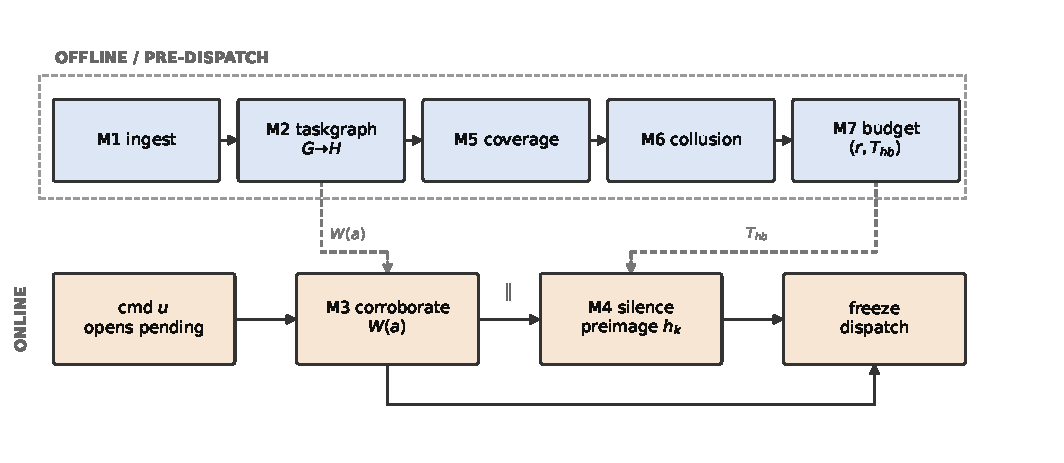
\includegraphics[width=0.92\textwidth]{fig/fig_architecture.pdf}
  \Description{Offline modules M1--M7 and online corroboration parallel silence pipeline.}
  \caption{方法总图（M1--M7）。离线导出见证集与 $(r,T_{\mathrm{hb}})$；在线 M3 与 M4 并行合用。}
  \label{fig:architecture}
\end{figure*}

\subsection{耦合互证}
\label{sec:corr}

由 BPMN 导出任务图 $G$，将跨设备类、同位置的交付--取件对构成互证超图 $H$，活动 $a$ 的见证集
\[
  W(a)=\{d'\in\mathcal{D}: d'\text{ 与 }a\text{ 在 }H\text{ 上物理耦合}\}.
\]
Trier 上见证边 185 条，中位 $|W|{=}1$，最大 6。
协议采用双截止：看门狗截止（命令打开）与互证截止（对手方确认窗口），时序见图~\ref{fig:protocol}；判定过程见算法~\ref{alg:corr}。
结果为确认、显式否证或逾窗判定；证据可转移归档。
\textbf{贡献在选取原则}：同协议对象下仅替换见证策略即可对照地理邻居、随机提名、全网询证与 PBFT 式法定人数（第~\ref{sec:eval}~节第二档）。

互证时延受派发排队支配（本日志排队 p95 约 218\,s，容差取 260\,s），故只有\textbf{条件}上界——在对手方被派发之后；不代入功能安全时间预算。

\begin{figure}[t]
  \centering
  
\includegraphics[width=\columnwidth]{fig/fig_protocol.pdf}
  \Description{Timeline of command-opened dual deadlines and heartbeat preimage slots.}
  \caption{协议时序：命令打开双截止互证窗口；心跳槽与调度队列解耦。}
  \label{fig:protocol}
\end{figure}

\begin{algorithm}[t]
\caption{耦合互证（调度器侧）}
\label{alg:corr}
\begin{algorithmic}[1]
\Require 命令账本 $c$，超图 $H$，容差 $\Delta$
\Upon{收到下行派工 $u$ 写入 $c$}
  \State 打开 pending$(u)$；$W\!\leftarrow\!W(u)$；$t_{\mathrm{wd}},t_{\mathrm{corr}}\!\leftarrow\!$ 双截止
\EndUpon
\Upon{收到完成声明 $r$ 或对手方确认/否证}
  \If{对手方 $d'\!\in\!W$ 显式否证}
    \State 归档 \textsc{Refuted}；冻结相关派单
  \ElsIf{在 $t_{\mathrm{corr}}$ 前收齐确认}
    \State 归档 \textsc{Confirmed}
  \ElsIf{逾 $t_{\mathrm{wd}}$ 或 $t_{\mathrm{corr}}$ 且声明已到达}
    \State 归档 \textsc{Expired}（误报分母仅计此类）
  \EndIf
\EndUpon
\end{algorithmic}
\end{algorithm}

\subsection{可问责沉默}
\label{sec:silence}

设备以 Ed25519 签名注册承诺根 $R_d$，绑定身份与会话；哈希链 $h_0,h_1,\dots$ 满足 $h_k=H(h_{k+1})$，元素与槽号一一对应。
槽 $k$ 截止须披露原像 $h_k$，语义为``槽内状态仍落在预测带内''（算法~\ref{alg:silence}）。
连续 $r$ 个槽缺失则确定性判定。
与 TESLA 的关键差别：链上原像直接作为一次性凭证，而非披露后失效的 MAC 密钥。

\begin{algorithm}[t]
\caption{可问责沉默（调度器侧）}
\label{alg:silence}
\begin{algorithmic}[1]
\Require 已注册根 $R_d$，间隔 $T_{\mathrm{hb}}$，阈值 $r$，时钟 skew 上界 $\varepsilon$
\State 槽 $k$ 的截止时刻 $t_k^\star \leftarrow t_0 + k T_{\mathrm{hb}}+\varepsilon$
\Upon{时刻 $t_k^\star$}
  \If{已收到通过 $R_d$ 验证的原像 $h_k$}
    \State 重置缺失计数
  \Else
    \State 缺失计数 ${+}\!1$；若 $\ge r$ 则判定可问责沉默并冻结派单
  \EndIf
\EndUpon
\end{algorithmic}
\end{algorithm}

\begin{proposition}[原像披露的不可否认性（归约草图）]
\label{prop:nr}
设（i）$R_d$ 由设备私钥对 $\langle\mathrm{id},\,\mathrm{session},\,h_0\rangle$ 签名锚定；（ii）槽号与链元素一一绑定；（iii）松散同步保证接收方对截止 $t_k^\star$ 的判定一致。
则任何第三方持有 $(R_d,h_k)$ 均可验证``$h_k$ 只能由承诺者产生''；攻击者若在截止后伪造合法 $h_k$，则可破哈希单向性或伪造 Ed25519 签名。
\end{proposition}
\begin{proof}[草图]
验证即检查签名绑定与 $H^{(k)}(h_k)=h_0$。
若敌手在不知 $h_{k+1}$ 时输出通过验证的 $h_k'$，则给出对 $H$ 的原像；若改绑定身份，则需伪造根签名。
与 TESLA 不同，披露后第三方\emph{不能}用已公开密钥重算 MAC 冒充源，因为凭证本身即原像而非对称密钥。
完整归约见附录（投稿版可展开）。
\end{proof}

心跳与调度队列解耦，故 $T_{\mathrm{detect}}\le r\,T_{\mathrm{hb}}$ 为\textbf{无条件}上界（检测回放口径下中位约 1.8\,s），接入第~\ref{sec:theory}~节定理。

\subsection{合用与归因}
\label{sec:compose}

仅互证：对 P2 沉默仍可因命令开窗而超时检出，但时延中位达数百秒，且无法代入无条件 FHI 预算。
仅沉默：P3 按时披露原像同时谎报完成，DR${=}0$——这是互证不可被替代的直接证据。
合用后无获胜支：P1/P2 由沉默压到约 1.8\,s，P3 由互证兜住。
另有实测收益：沉默设备会拒绝为上游作证，导致诚实上游声明超时；沉默通道直接指认沉默者，避免冤枉上游。

\subsection{覆盖与串谋界的设计面}
\label{sec:covdesign}

无对手方区间可用按需主动互证探测补洞；先知传感器天花板给出覆盖缺口上界（约 $29.95\%$）。
串谋界可反用为派工约束（只下发互证路径足够长的分解）：实测可改善分布均值，但抬不动最小值与中位时须诚实陈述，不可写成提高了安全保证下界。

\subsection{复杂度与密码预算}
\label{sec:budget_eng}

每条完成声明查 $W(a)$（中位 $O(1)$）并作常数次验签/归档；每槽一次原像披露与哈希核对。
带宽 $n L/T_{\mathrm{hb}}$ 由预算反解。
高频路径用链路层认证 + MAC，可问责沉默用哈希链令牌，稀有事件与视图切换才用签名。

%=============================================================================
\section{理论分析}
\label{sec:theory}

\subsection{串谋界}
\label{sec:collusion}

在互证超图上定义``下一对手方''关系的前向可达闭包。
要使谎言存活至物料被消耗，联盟须覆盖闭包上每一跳。
形式化对象是该闭包长度 $k$，而非最小顶点割。
Trier 上实测 $k_{\min}{=}1$、中位 $5$、最大 $13$，$k\ge 3$ 约占 $81\%$。
一跳串谋（P4）只推迟判决：主受害者可因串谋方背书而通过，串谋方随后交付仍被下游诚实设备否证。
图~\ref{fig:collusion} 给出作用域内链的 $k$ 直方图。

\begin{figure}[t]
  \centering
  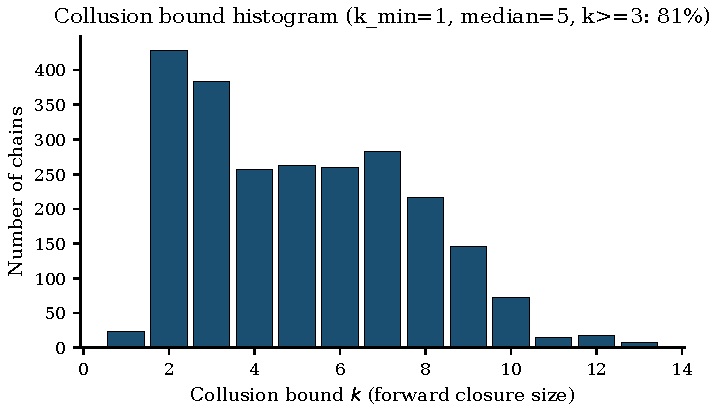
\includegraphics[width=\columnwidth]{fig/fig_collusion.pdf}
  \Description{Histogram of collusion bound k over in-scope chains.}
  \caption{串谋界 $k$ 的分布（前向闭包；数据由 \texttt{tessera} 现场导出）。}
  \label{fig:collusion}
\end{figure}

\subsection{带宽--安全裕度权衡}
\label{sec:bw}

待界定量取沉默通道的 $T_{\mathrm{detect}}\le r\,T_{\mathrm{hb}}$（互证窗口 $\Delta$ 受排队支配、无上界，不得代入）。
四段链条（图~\ref{fig:budget-chain}）：
\[
  \text{危害模型}\;\longrightarrow\;\text{时间预算}\;\longrightarrow\;(r,T_{\mathrm{hb}})\;\longrightarrow\;\text{带宽下界}.
\]

\begin{figure}[t]
  \centering
  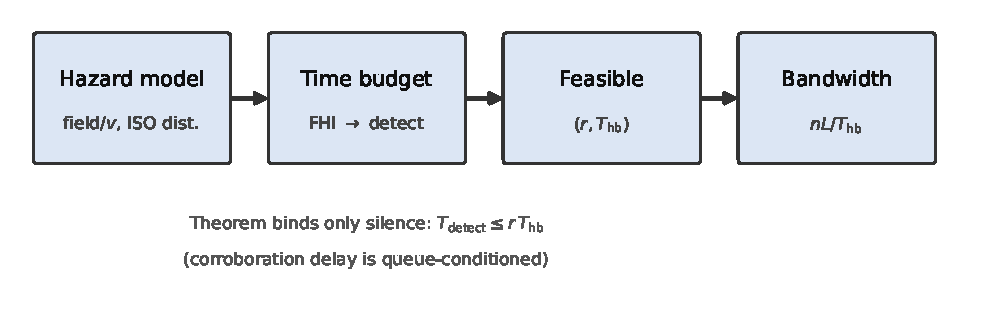
\includegraphics[width=\columnwidth]{fig/fig_budget_chain.pdf}
  \Description{Four-stage chain from hazard model to bandwidth lower bound.}
  \caption{带宽--安全裕度四段链。定理只接沉默通道的无条件时延上界。}
  \label{fig:budget-chain}
\end{figure}

直接借用汽车领域 FHI${=}2.43$\,s 会导致假合规：留给检测的时间可使低速 AGV 驶出防护场。
应由危害模型反推，例如防护场 $1.275$\,m、$v{=}1.5$\,m/s 时 $\mathrm{FHI}{=}\mathrm{field}/v{=}0.85$\,s。
ISO~13855 / 3691-4 的距离公式作为第一段输入~\cite{iso13855,iso3691}；主威胁是调度损害时，该换算用于校准预算量级而非充当安全论断。

\begin{theorem}[带宽受安全约束限制]
\label{thm:bw}
给定设备数 $n$、单槽载荷 $L$、误报预算 $\Lambda$（次/小时）与丢包模型（独立或突发相关系数 $\rho$），
设危害模型导出检测段预算 $T_{\mathrm{budget}}$。
若存在整数 $r\ge 1$ 与 $T_{\mathrm{hb}}>0$ 使
（a）$r\,T_{\mathrm{hb}}\le T_{\mathrm{budget}}$，且
（b）在该丢包模型下槽缺失误报率 $\le\Lambda$，
则取满足（a）（b）的最大 $T_{\mathrm{hb}}$ 时，心跳带宽下界为 $B^\star=n L/T_{\mathrm{hb}}$。
若该最优点使（a）以等号成立而（b）仍有松弛，则称带宽受安全约束限制。
\end{theorem}
\begin{proof}[草图]
沉默判定至多等待 $r$ 个槽，故 $T_{\mathrm{detect}}\le r\,T_{\mathrm{hb}}$；要求其不超过 $T_{\mathrm{budget}}$ 即得（a）。
误报由丢包导致的虚假缺失决定：独立丢包下可用二项尾，突发下用相关模型抬高有效 $r$（实现见 \texttt{budget.py}）。
在可行集上极大化 $T_{\mathrm{hb}}$ 等价于极小化 $B=nL/T_{\mathrm{hb}}$。
最优落在（a）边界当且仅当安全预算比误报预算更紧——这是``带宽受安全约束''的操作化定义，可由求解器返回的 binding 标签核验。
互证窗口 $\Delta$ 不含于本定理：其由派发排队支配、无通用上界。
\end{proof}

实测（28 台设备、丢包 1\%、误报预算 1 次/h）：突发容忍相对独立丢包约 $3.32\times$ 带宽代价；预算由汽车口径收紧至运动危害约 $4.59\times$；最严口径（运动危害 + 突发）$7675$\,B/s，仍为 5\,Hz PBFT 量级的 $1/131$。
FHI、反应时间与丢包率为引用或仿真参数（Trier 无 AGV/通信层），须在表注标注来源。

%=============================================================================
\section{实验评估}
\label{sec:eval}

\subsection{实验设置}
\label{sec:setup}

\textbf{主数据：}Fischertechnik Trier IoT 事件日志 + 16 个 BPMN~\cite{trier2022}，自建攻击注入器 P1--P4（默认注入率 0.2、种子 42）。
\textbf{叙事/数据/参数分离：}AGV 叙事只用于威胁说明；心跳与 FHI 参数非本日志实测。
\textbf{指标：}检出率（DR）、误报率（FAR）、判别力、检测时延、见证集规模、串谋界 $k$、带宽。
\textbf{铁律：}每次对比声明等带宽或等误报率。
基线按\textbf{消耗的信息}分档，不按论文分组。
\textbf{复现：}协议与基线实现于开源原型 TESSERA（\texttt{paper03/tessera}）；一键入口 \texttt{py main.py}，断言集 \texttt{tests/test\_all.py}（63 条）锚定本文主表数字。

\subsection{第一档：单观测者结构性失效}
\label{sec:tier1}

伪造声明在单观测者可见字段上可与良性一致。
看门狗 S1、计划一致性残差 S2（通用 FDI 类）、对齐式过程一致性 S3 对 P1/P3 检出为结构性 0（或判别力约 0）；对 P2 能发现沉默。
该档证明必须引入物理对手方，不是与本文赛马（图~\ref{fig:tier1}）。

\begin{figure}[t]
  \centering
  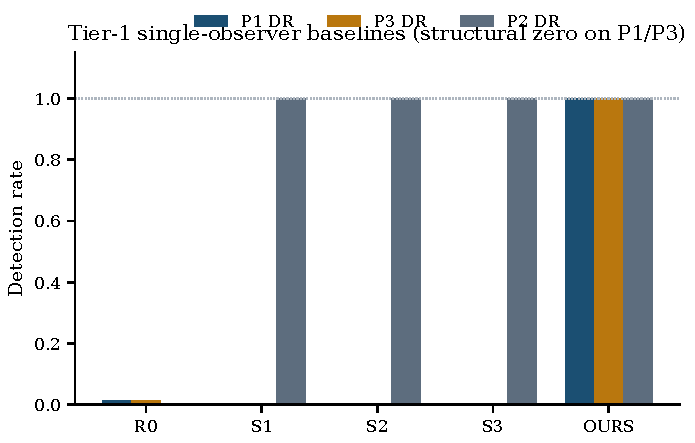
\includegraphics[width=\columnwidth]{fig/fig_tier1.pdf}
  \Description{Bar chart of tier-1 baseline detection rates on P1 P2 P3.}
  \caption{第一档基线：单观测者族对 P1/P3 结构性失效，对 P2 仍可发现沉默。}
  \label{fig:tier1}
\end{figure}

\begin{table}[t]
  \centering
  \caption{第一档基线（P1；与本文同窗口口径）}
  \label{tab:tier1}
  \begin{tabular}{@{}lcccc@{}}
    \toprule
    方法 & FAR & P1 DR & P3 DR & P2 DR \\
    \midrule
    S1 看门狗 & 0.042 & 0.000 & 0.000 & 1.000 \\
    S2 计划残差 & 0.004 & 0.003 & 0.003 & 1.000 \\
    S3 一致性检验 & 0.000 & 0.000 & 0.000 & 1.000 \\
    \textbf{耦合互证} & 0.023 & \textbf{1.000} & \textbf{1.000} & 1.000 \\
    \bottomrule
  \end{tabular}
\end{table}

\subsection{第二档：见证选取原则（主结果）}
\label{sec:tier2}

同一互证协议、同一窗口与容差，仅替换见证策略（图~\ref{fig:witness}）：

\begin{figure*}[t]
  \centering
  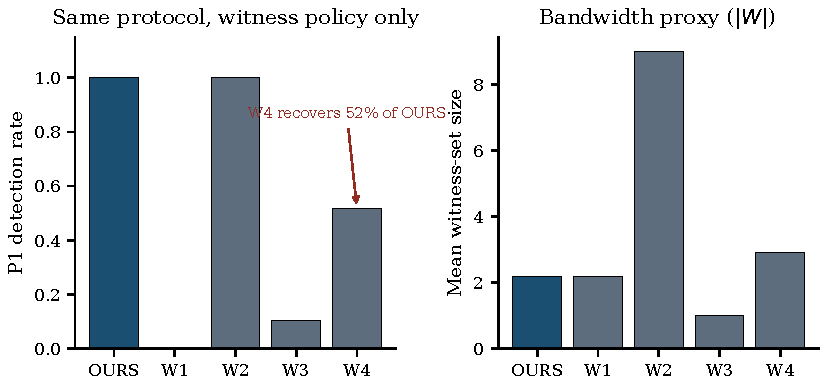
\includegraphics[width=0.88\textwidth]{fig/fig_witness.pdf}
  \Description{P1 detection rate and mean witness set size for OURS and W1--W4.}
  \caption{第二档主结果：同协议下只换见证选取。空间邻居（W4）约恢复本文 52\% 检出且见证集更大。}
  \label{fig:witness}
\end{figure*}

\begin{table}[t]
  \centering
  \caption{第二档：同协议下见证选取对照（P1）}
  \label{tab:tier2}
  \begin{tabular}{@{}lccc@{}}
    \toprule
    策略 & DR & 相对 $|W|$ 均值 & 备注 \\
    \midrule
    W1 PBFT 式法定人数 & 0.000 & ${\approx}1\times^{\dagger}$ & 无物理证据 \\
    W2 全体询证 & ${\approx}$本文 & $4.13\times$ & 零增益 \\
    W3 随机 $k$ 见证 & 0.105 & ${\approx}1\times$ & 崩塌 \\
    W4 空间邻居 & ${\approx}0.52$ & $1.34\times$ & 主对照 \\
    \textbf{任务图 $W(a)$} & \textbf{1.000} & $1\times$ & 本文 \\
    \bottomrule
  \end{tabular}
  \begin{tablenotes}
    \item $^{\dagger}$W1 的见证集规模与本文同为均值 2.18；其额外代价是全网共识消息带宽约为沉默心跳的 $131\times$，不是 $|W|$ 放大。
  \end{tablenotes}
\end{table}

头条主张：贡献在任务图选取原则；``更多见证者''或``有见证''本身不够。W1 说明付高带宽换一致性仍检不出任务状态伪造。

\subsection{消融与覆盖矩阵}
\label{sec:ablation}

表~\ref{tab:coverage} 即消融；热力图见图~\ref{fig:ablation}：去掉互证则 P3 完全逃脱；去掉沉默则 P1/P2 时延恶化一到两个数量级。

\begin{figure}[t]
  \centering
  
\includegraphics[width=\columnwidth]{fig/fig_ablation.pdf}
  \Description{Heatmap of detection rate and latency across attacks and channels.}
  \caption{消融/覆盖矩阵热力图（格内为 DR 与时延中位）。P3 行表明互证不可替代。}
  \label{fig:ablation}
\end{figure}

\subsection{第三、四档与预算扫参}
\label{sec:tier34}

等带宽周期性全量上报（H1）时延约 $8\times$，最严口径超出检测预算（图~\ref{fig:heartbeat}）；无密码绑定的 GOOSE 式心跳（H2）有活性无归责；TESLA 式延迟密钥（H3）披露后可伪造，归责失败。
先知传感器预言机（U1）覆盖 100\%，相对实现覆盖的缺口约 $29.95\%$（图~\ref{fig:coverage}）。
沉默带宽相对 5\,Hz PBFT 的倍数见图~\ref{fig:budget-bw}；丢包率扫参见图~\ref{fig:loss}（含 $p{=}50\%$ 地标，突发下约 $27502$\,B/s）。

\begin{figure}[t]
  \centering
  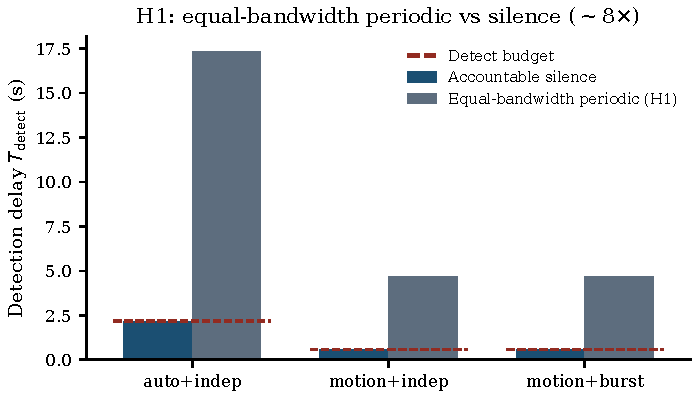
\includegraphics[width=\columnwidth]{fig/fig_heartbeat.pdf}
  \Description{Equal-bandwidth periodic detection delay versus accountable silence.}
  \caption{第三档 H1：等带宽周期全量上报的检测时延约为沉默通道的 $8\times$，且超出运动危害检测预算。}
  \label{fig:heartbeat}
\end{figure}

\begin{figure}[t]
  \centering
  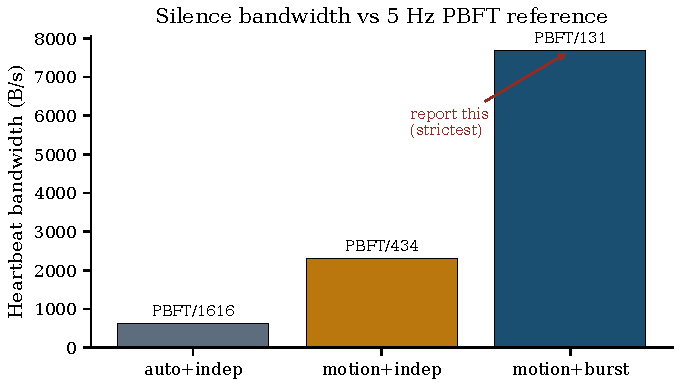
\includegraphics[width=\columnwidth]{fig/fig_budget_bw.pdf}
  \Description{Silence heartbeat bandwidth under three regimes versus PBFT ratio.}
  \caption{可问责沉默心跳带宽。论文应报最严口径（运动+突发，$\approx$ PBFT$/131$）。}
  \label{fig:budget-bw}
\end{figure}

\begin{figure}[t]
  \centering
  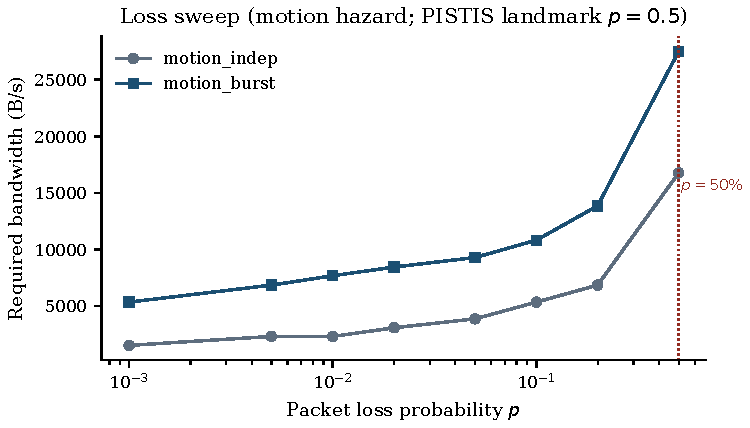
\includegraphics[width=\columnwidth]{fig/fig_loss_sweep.pdf}
  \Description{Required bandwidth versus packet loss probability.}
  \caption{丢包率扫参（数据：\texttt{tessera/experiments/loss\_sweep.csv}）。}
  \label{fig:loss}
\end{figure}

\begin{figure}[t]
  \centering
  
\includegraphics[width=\columnwidth]{fig/fig_coverage.pdf}
  \Description{Fraction of activities corroborated versus oracle gap.}
  \caption{第四档 U1：先知覆盖与实现覆盖之差即按需主动互证靶区。}
  \label{fig:coverage}
\end{figure}

%=============================================================================
\section{局限与结论}
\label{sec:conclusion}

\subsection{局限}

需要松散时间同步与有界心跳，否则归责退回异步不可归因困境。
同一超边上对手方同时被劫持时，该跳互证失效——这是应由串谋界量化的边界，不是实现缺陷。
不假设 TEE，故不检测软件篡改本身，只检测其在任务状态上的外显后果。
存在无对手方覆盖缺口；FHI/丢包非 Trier 实测；主危害是调度损害。

\subsection{结论}

本文针对被劫持设备的任务状态伪造，提出任务图诱导的耦合互证与不依赖分歧的可问责沉默，并给出带宽--安全裕度权衡。
Trier 实验表明：单观测者族对无残差伪造结构性失效；见证选取原则决定检出能力；P3 证明互证不可替代；最严心跳带宽仍较周期性全网 PBFT 低两个数量级。
部署含义：$T_{\mathrm{hb}}$ 由安全预算解出；见证按任务图配置。
未来工作包括在柔性车间上最大化互证覆盖的派工，以及实网丢包与时间同步标定。

%=============================================================================
\begin{thebibliography}{99}

\bibitem{pistis2021}
D.~Kozhaya, J.~Decouchant, and P.~Esteves-Verissimo,
``PISTIS: An Event-Triggered Real-Time Byzantine-Resilient Protocol Suite,''
\textit{IEEE Trans. Parallel Distrib. Syst.}, vol.~32, no.~9, pp.~2271--2286, 2021.

\bibitem{tac2025el}
``Event-Triggered Resilient Consensus of Networked Euler--Lagrange Systems Under Byzantine Attacks,''
\textit{IEEE Trans. Autom. Control}, 2025, doi:10.1109/TAC.2025.3582531.

\bibitem{hdetm2024}
``A robust control framework for multi-agent systems under Byzantine attacks using hybrid event-triggered techniques,''
\textit{Ain Shams Eng. J.}, 2024, doi:10.1016/j.asej.2024.103149.

\bibitem{ccgridw2023pbft}
``An Improved PBFT-Based Consensus Protocol for Industrial IoT,''
in \textit{Proc. CCGridW}, 2023, doi:10.1109/CCGridW59191.2023.00068.

\bibitem{sensors2024aloha}
``Slotted ALOHA Based PBFT Blockchain Networks: Performance Analysis and Optimization,''
\textit{Sensors}, vol.~24, no.~23, p.~7688, 2024.

\bibitem{nontrigger2022}
``Performance Analysis of Event-Triggered Consensus Control for Multi-agent Systems under Cyber-Physical Attacks,''
\textit{arXiv:2201.02997}, 2022.

\bibitem{asjc2023contain}
``Event-triggered containment control for multi-agent systems under hybrid cyber attacks,''
\textit{Asian J. Control}, 2023, doi:10.1002/asjc.3180.

\bibitem{ijrnc2023deception}
``Event-triggered control of Takagi--Sugeno fuzzy systems under deception attacks,''
\textit{Int. J. Robust Nonlinear Control}, 2023, doi:10.1002/rnc.6760.

\bibitem{peerreview2007}
A.~Haeberlen, P.~Kuznetsov, and P.~Druschel,
``PeerReview: Practical Accountability for Distributed Systems,''
in \textit{Proc. SOSP}, 2007, pp.~175--188.

\bibitem{polygraph2021}
P.~Civit, S.~Gilbert, and V.~Gramoli,
``Polygraph: Accountable Byzantine Agreement,''
in \textit{Proc. ICDCS}, 2021, pp.~403--413.

\bibitem{abc2023}
P.~Civit, S.~Gilbert, V.~Gramoli, et~al.,
``As easy as ABC: Optimal Accountable Byzantine Consensus is easy!,''
\textit{J. Parallel Distrib. Comput.}, vol.~181, 2023.

\bibitem{tesla2001}
A.~Perrig, R.~Canetti, J.~D.~Tygar, and D.~Song,
``Efficient Authentication and Signing of Multicast Streams over Lossy Channels,''
in \textit{Proc. IEEE Symp. Security and Privacy}, 2000.

\bibitem{rfc4082}
A.~Perrig, D.~Song, R.~Canetti, J.~D.~Tygar, and B.~Briscoe,
``Timed Efficient Stream Loss-Tolerant Authentication (TESLA),''
RFC~4082, 2005.

\bibitem{inftesla2022}
``Enhanced Inf-TESLA Protocol,''
\textit{IEEE Access}, 2022, doi:10.1109/ACCESS.2022.3177268.

\bibitem{goose615}
ABB,
``IEC 61850 Engineering Guide: 615 series,''
technical manual (GOOSE MaxTime / TAL heartbeat semantics).

\bibitem{diat2019}
T.~Abera, R.~Bahmani, F.~Brasser, et~al.,
``DIAT: Data Integrity Attestation for Resilient Collaboration of Autonomous Systems,''
in \textit{Proc. NDSS}, 2019.

\bibitem{colaw2020}
P.~Barabas, E.~Regnath, and S.~Steinhorst,
``COLAW: Cooperative Location Proof Architecture for VANETs based on Witnessing,''
in \textit{Proc. COINS}, 2020, doi:10.1109/COINS49042.2020.9191402.

\bibitem{vouch2019}
F.~Boeira, M.~Asplund, and M.~Barcellos,
``Decentralized proof of location in vehicular ad hoc networks,''
\textit{Comput. Commun.}, vol.~147, pp.~98--110, 2019.

\bibitem{etsi460}
ETSI,
``Intelligent Transport Systems; Security; Pre-standardization study on Misbehaviour Detection,''
ETSI TR 103 460 V2.1.1.

\bibitem{ditof2024}
J.~Bahrami, M.~Ebrahimabadi, M.~Younis, and N.~Karimi,
``Digital Twin Based Topology Fingerprinting for Detecting False Data Injection Attacks in Cyber-Physical Systems,''
in \textit{Proc. IEEE ICC}, 2024, pp.~2053--2058.

\bibitem{dtmpc2025}
``Digital Twin-Based Resilient Model Predictive Control for Industrial Cyber-Physical Systems,''
\textit{IEEE J. Emerg. Sel. Topics Ind. Electron.}, 2025, doi:10.1109/JESTIE.2025.3528881.

\bibitem{agvkpi2022}
``Detecting and Processing Anomalies in a Factory of the Future,''
\textit{Appl. Sci.}, vol.~12, no.~16, p.~8181, 2022.

\bibitem{fdi2024frontiers}
``An evaluation of methods for detecting false data injection attacks in the smart grid,''
\textit{Frontiers Comput. Sci.}, 2024.

\bibitem{cn120578205b}
``一种抗虚假数据注入攻击的多 AGV 事件触发安全路径跟踪方法,''
中国专利 CN120578205B.

\bibitem{usaid}
A.~Ibrahim, A.-R.~Sadeghi, and G.~Tsudik,
``US-AID: Unattended Scalable Attestation of IoT Devices,''
in \textit{Proc. IEEE SRDS}, 2018, pp.~21--30.

\bibitem{trier2022}
L.~Malburg, J.~Gr\"uger, and R.~Bergmann,
``An IoT-Enriched Event Log for Process Mining in Smart Factories,''
\textit{arXiv:2209.02702}, 2022.

\bibitem{iso13855}
ISO~13855,
``Safety of machinery --- Positioning of safeguards with respect to the approach speeds of parts of the human body.''

\bibitem{iso3691}
ISO~3691-4:2023,
``Industrial trucks --- Safety requirements and verification --- Part~4: Driverless industrial trucks.''

\end{thebibliography}

\end{document}
